\pagebreak
\subsection{Moment of Inertia} %\label{put a label here and uncomment}
\textbf{Name: Group 510}\\
\textbf{Date: 30/09 - 2015}

\subsubsection{Purpose}
The purpose of this test is to find the moment of inertia $I$, by measuring the motor velocity as a function of time.

\subsubsection{Setup}
\begin{figure}[H]
  \centering
	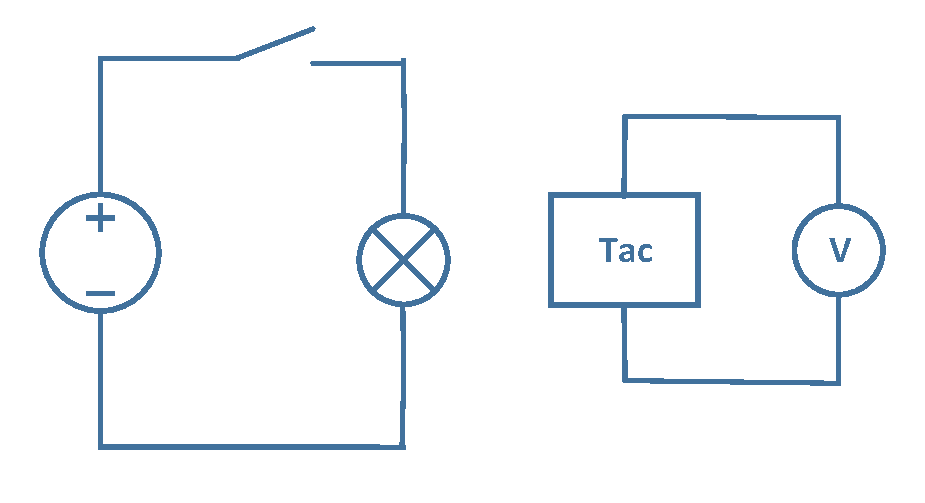
\includegraphics[scale=0.5]{figures/MotorTest7.pdf}
	\caption{Setup diagram}
\end{figure}

\subsubsection{List of Equipment}

\begin{table}[H]
\begin{tabular}{|l|l|p{4cm}|}
\hline%------------------------------------------------------------------------------------
  \textbf{Instrument}                        &  \textbf{AAU-no.}  &  \textbf{Type}       \\
\hline%------------------------------------------------------------------------------------
  Oscilloscope                               &  64672             &  Agilent DSO6034A    \\
\hline%------------------------------------------------------------------------------------
  Power Supply ($0 - 32$ V) ($0 - 10$ A)     &  77076             &  Ea - ps 7032 - 100  \\
\hline%------------------------------------------------------------------------------------
  Optical tachometer                         &  77087             &  Compact             \\
\hline%------------------------------------------------------------------------------------
\end{tabular}
\end{table}

\subsubsection{Procedure}

\begin{enumerate}
  \item Turn on the oscilloscope, and connect the tachometer to one of the inputs.
  \item On the oscilloscope press the "trigger mode"-key choose the "normal"-option, set the trigger to "falling edge".
  \item To prevent false triggering on the oscilloscope set the trigger value to \num{1,175} V with the turn-key.
  \item Turn on the power supply at 7 volt.
  \item Press "single"-key on oscilloscope and cut the power of the motor.
  \item Insert a USB-flash drive in the oscilloscope and press the save key to extract the data.
\end{enumerate}

\subsubsection{Results}

\begin{figure}[H]
  \setcounter{subfigure}{0}
  \centering
  \begin{subfigure}{0.45\textwidth}
    \centering
    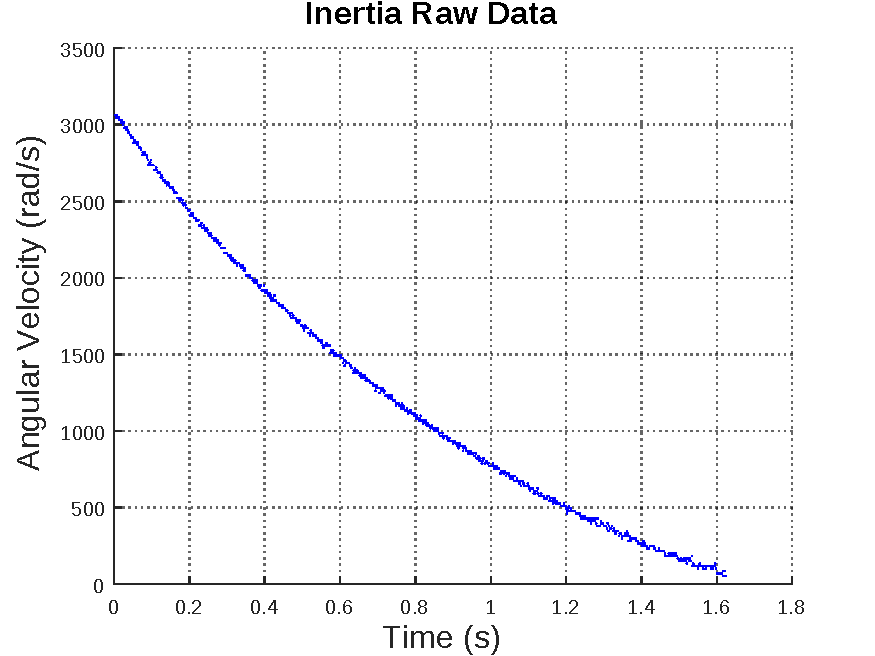
\includegraphics[width=1.1\linewidth]{figures/inertiaRawData.pdf}
    \caption{The measured angular velocity compared to time}
    \label{inertiaRawData}
  \end{subfigure}
  \begin{subfigure}{0.45\textwidth}
    \centering
    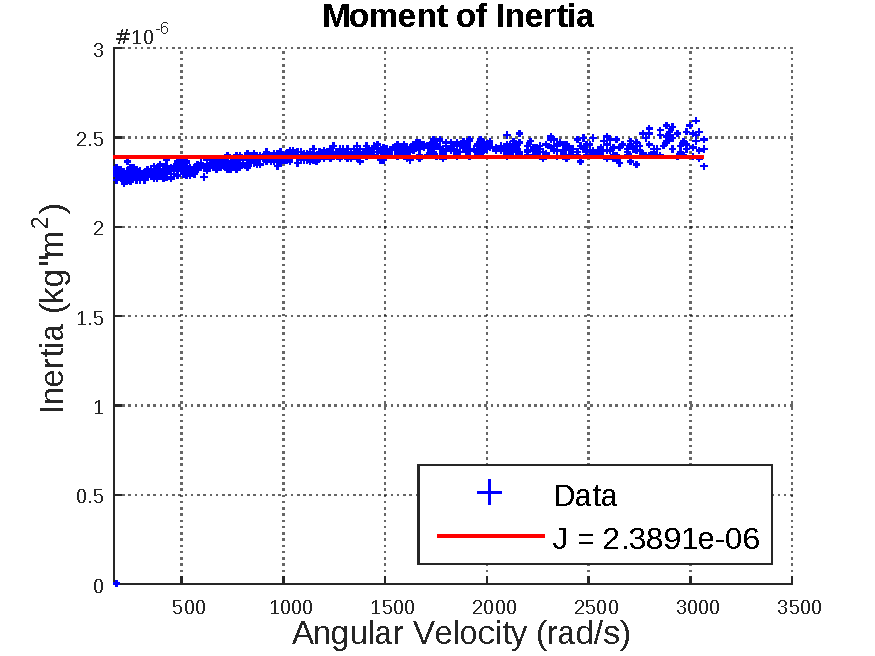
\includegraphics[width=1.1\linewidth]{figures/momentOfInertia.pdf}
    \caption{Blue dots indicates the moment of inertia calculated using \eqref{eq:Momentofinertia}, and the red line represents the average value of the blue dots}
  	\label{momentOfInertia}
  \end{subfigure}
  \caption{A plot of the inertia measured as angular velocity compared to time and a plot of the moment of inertia calculated from the raw data using \eqref{eq:Momentofinertia}.}
  \label{yo}
\end{figure}
\todo{make text on figure larger}

The equation used is given in the Modeling and Control course on the 5th semester on Electronic and IT on Aalborg University, (reference). This equation which arises from the mechanical description of the motor, when \si{i_a = 0} is used to find the Inertia, J.
\begin{align}
  \eq{\omega(s)}{- \frac{\tau_c}{B}+(\omega_0 + \frac{\tau_c}{B}) e^{-t\frac{B}{J}}} \unit{rad\cdot s^{-1}}\nonumber\\
  && &\Updownarrow&&\\
  \eq{J}{ \frac{B\cdot t}{ln(  \frac{B\cdot \omega_0 + \tau_c}{B \cdot \omega + \tau_c})} } \unit{N\cdot m}\nonumber
 \label{eq:Momentofinertia}
\end{align}
\hspace{6mm} Where:\\
\begin{tabular}{p{1cm}ll}
& \si{\omega(s)} & is the angular velocity [$\frac{rad}{s}$] \\
& \si{\tau_c} & is the coulomb friction torque [$N \cdot m$]\\
& B & is the friction [$N \cdot m$] \\
& J & is the inertia [$Kg \cdot m^2$] \\
\end{tabular}

The motors inertia is calculated by using \eqref{eq:Momentofinertia} on the angular velocity compared to time data illustrated on \figref{inertiaRawData}. Thereafter the average value of the results is found, seen in \figref{momentOfInertia} and used a the motors inertia. The motors inertia is equal:

\begin{align}
\eq{J}{\num{2.3891} \cdot 10^{-6}} \unit{Kg \cdot m^2}
 \label{eq:Momentofinertia}
\end{align}


